
% ibs.tex

\documentclass[10pt,a4paper,titlepage]{article}
\usepackage[czech]{babel}
\usepackage[utf8]{inputenc}
\usepackage[margin=100pt]{geometry}
    
\usepackage{graphicx}   % Import pictures
\usepackage{multicol}
\usepackage{caption}
\usepackage{subcaption}
%\usepackage{csquotes}

\usepackage[backend=biber, sorting=none]{biblatex}
\addbibresource{ibs.bib}
    
\begin{document}
  \pagenumbering{gobble}

  \begin{center}
    \section*{Analýza komunikace Facebook a Twitter}
    Martin Beneš
  \end{center}

  \section*{Úvod}
  Sociální sítě jsou dnes skutečným fenoménem. K roku 2018 hlásí nejpopulárnější
  síť Facebook přes~2 miliardy aktivních uživatelů, využívá jej každý druhý čech.
  Za~ní zůstavá YouTube, spadající pod~Google, s~1.5 milardy,
  třetím jsou WhatsApp a Facebook Messenger, obě vlastnictvím Facebook~Inc.,
  čítající 1.3 miliardy uživatelů. Další u nás populární sítě dnešní doby
  jsou Instagram (800~mil.), Twitter (330~mil.), Skype (300~mil.) a další. \cite{UserCount}

  %Ať již chceme nebo ne, k zadaným osobním údajům (jménu, fotografiím,
  %videím, zprávám) má daná síť přístup, a to podle podmínek, které se sama
  %stanovuje a se kterými musíte souhlasit při registraci. Síť z tohoto
  %pohledu tedy než veřejné místo pro setkávání přípomíná spíše totalitní
  %zemi, kde si režim vezme, co se mu zlíbí, a nikdo s tím nic nemůže
  %udělat~-~ovšem s otevřenými hranicemi, nikdo uživatele nenutí být na Facebooku.

  Většina z~těchto platforem poskytuje aplikační rozhraní (API), které nabízí
  jednoduché získání dat. Konkrétně autentizace Facebook i Twitter API je
  založena na autorizačním frameworku {\it OAuth2}, který umožňuje
  aplikacím limitovaný přístup k~účtu uživatele. \cite{FacebookOauth} \cite{TwitterOauth}

  \subsection*{OAuth2}
  Protokol definuje 4 role: vlastníka zdrojů (uživatele), autorizační server
  a poskytovatele zdrojů (API) a klienta (aplikaci, která žádá o zdroje).

  \begin{figure}[h!]
    \begin{center}
      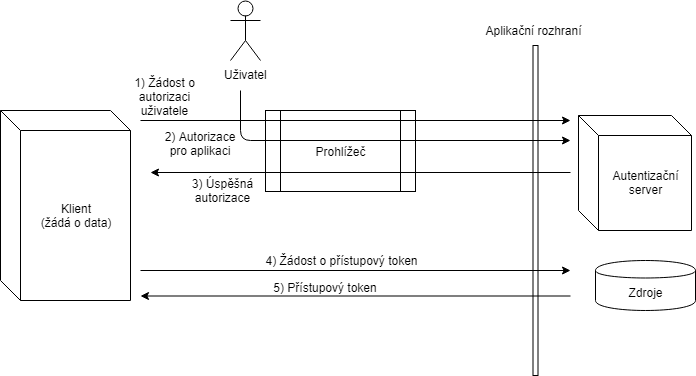
\includegraphics[width=0.6\textwidth]{oauth2.png}
      \caption[title=Obrazek]{Schéma protokolu OAuth2\label{fig:oauth2}}
    \end{center}    
  \end{figure}

  Klient nejprve odešle požadavek autorizačnímu serveru skrz API. Poté
  se uživatel autorizuje, a to přímo u autorizačního serveru pro
  zajištění důvěrnosti. Facebook v této fázi vyzve k povolení přístupu
  dané aplikace k profilu uživatele a zobrazí, o jaká data aplikace žádá,
  pouze tato data jí budou zpřístupněna. Klient následně obdrží od serveru
  autorizační kód, se kterým již přímo žádá o data. Sekvenční schéma protokolu
  je možné vidět na obrázku \ref{fig:oauth2}.
  
  \section*{Realizace útoku}

  \section*{Zhodnocení výsledků}
  Nakonec, největší úniky dat na Facebooku jsou vzhledem k nevědomosti,
  nebo nedbalosti uživatelů díky povolení přístupu aplikaci přímo uživatelem.
  Právě v dnešních dnech se okolo Facebooku točí velký skandál ohledně aféry
  s firmou Cambridge Analytica, která z Facebooku sesbírala data shruba
  87 milionů uživatel a zřejmě je použila pro ovlivnění voličů pří
  několikerých voleb v různých zemích. \cite{CambridgeAnalyticaScandal}


  
  
  % references
  \printbibliography

\end{document}